In this chapter, we will present the background and motivation of our thesis.
We start with our background in medical procedures, looking at how doctors perform colonoscopies, mainly from a gastrointestinal perspective.
Then will then look at what the objective is for the medical staff, with different anomalies in the GI tract. Then our focus is moved to how doctors use computer-aided diagnosis (CAD) today to help with the screening. Lastly, we look at current models for CAD made both by Simula.

After the discussion from a medical point of view, we shift our focus to machine learning and give a brief introduction to different machine learning methods. We will look at how machines can \'learn\' and discuss different areas we can use and areas we are using machine learning today.
We will then go in depth into the examples and look at the most common machine learning models. We will look at the most common form of machine learning, namely neural networks, and show the structure that is most used in this type of machine learning. 

 With this in mind, we will look
at neural networks, especially convolutional neural networks, and how they work.

Lastly, we will combine the need for computer-aided diagnosis with the machine learning.
\section{The Medical Background}
In the field of medical diagnosis, there are always new and interesting methods being researched to help the medical staff when it comes to patient \textit{rate of survival}, and quality of life. 
Everything from x to y is ways the medical industry has done to improve the survival rates of their patients. 
In the last decade \textit{comuters and cameras came to help us.}
Another example is the invention and usage of gastro-stick-with-camera.
\subsection{colonoscopy/gastro/procedure}
When performin gastronomi we use astik
\subsection{Medical images/data/other}
    
\subsection{Systems in place for detection}
\subsection{summary}
    

\section{Machine Learning}
We have looked at the challenges that the medical staff has when it comes to detecting polyps, and how it is solved today.
However, to truly understand how automated systems like Mirmir\todo{cite} works, we need to look at how Machine learning helps with the detection of the anomalies the medical staff are after.  

Machine learning is a broad term, but can, in short, be summarised by:\\
\vspace{10px}

\textit{ A computer program is said to learn from experience E with respect to some class of tasks T and performance measure P, if its performance at tasks in T, as measured by P, improves with the experience E. } \cite{MitchellTomM1997Ml}\\

\vspace{10px}
A few things of note from this quote is the variables mentioned in the quote. Experience e is the stored knowledge the program has gotten. It is in most cases just numbers used to approximate a solution given an input, to try to get it as close to the right answer. This approximation is made for every task T until we are happy with the result.
Lastly, to tell how well our program does we need a measure P that tells us how far away from the desired output we got.
   
From this, we see that the goal of machine learning is to improve some performance P with experience. This behaviour is a mimicry of human learning, where we as humans need to practice on a task to improve on it.
As the amount of experience increase, both for us and the machine, the performance of the task becomes better and better. With this in mind, we can assume that, given the right amount and type of data, our machine learning algorithms can solve any problems humans can solve, given both the right training environment and a way to train, given the environment.

We have talked about machine learning in broad terms at this point. We have drawn a parallel between how humans learn, and how machines gather experience.  Now we will look into the most popular machine learning techniques, and show the machine learning algorithms stores the experience gathered.
 
\subsection{Machine learning types}
With a basis in the quote from \cite{MitchellTomM1997Ml} \todo{fix}, we have a broad definition of what machine learning can be.
As long as we have a model trying to complete a task based on previous experience, it can be called machine learning. Though just like humans, we have multiple ways to gather and retain information.

Figure \ref{fig:ML_types} shows a chart over the three most common categories within the field of machine learning. 

    \begin{figure}[h]
        \centering
        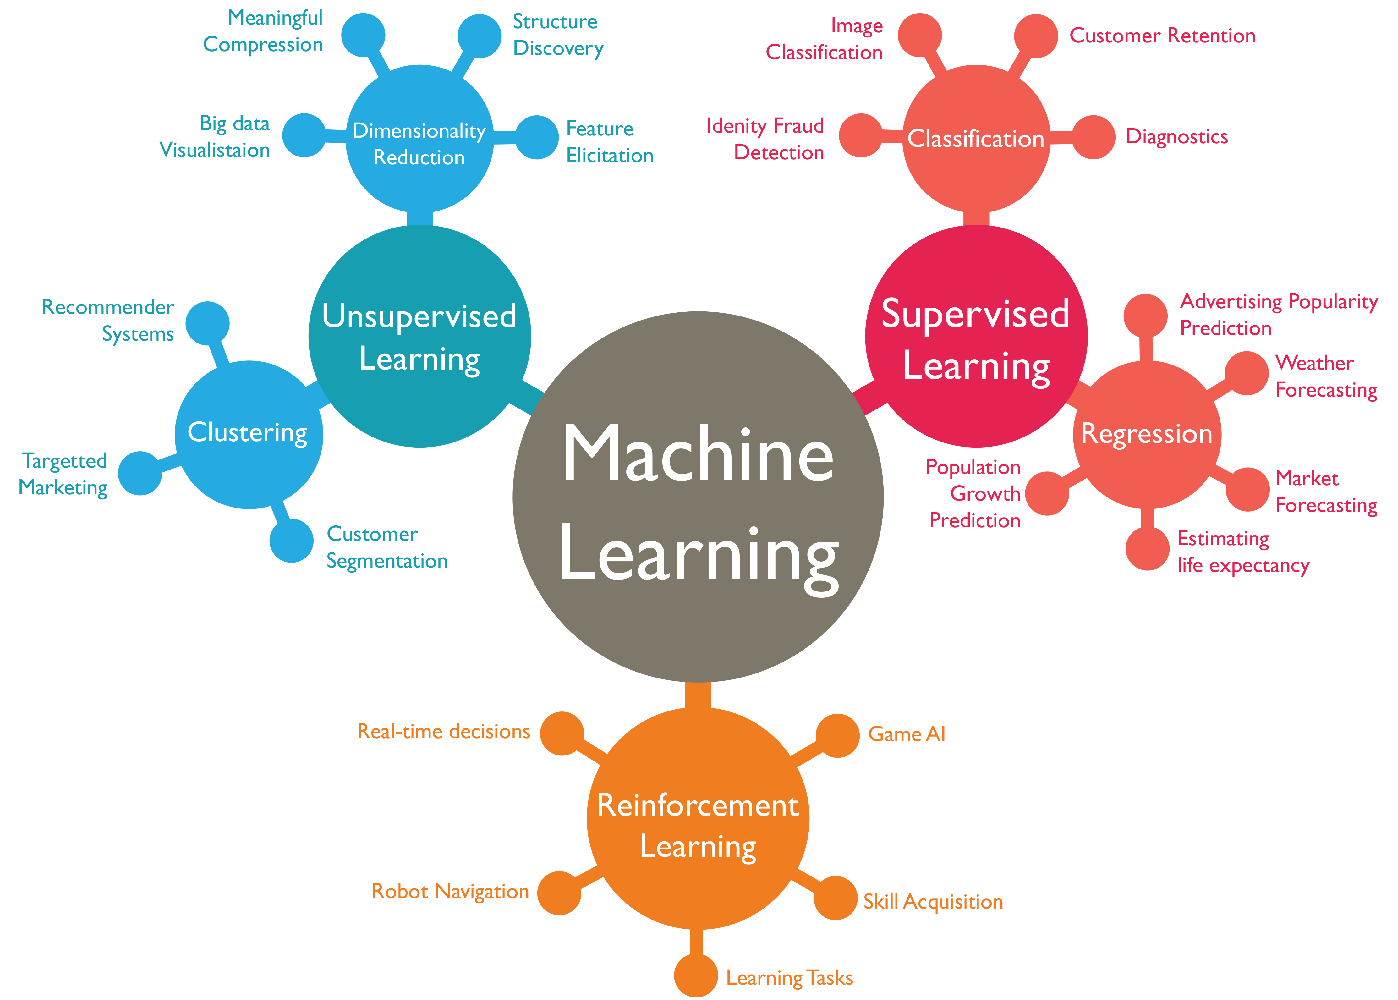
\includegraphics[scale=0.3]{background/figures/ML_types.png}
        \caption{The three main types of machine learning and their subtypes}
    \label{fig:ML_types} 
    \end{figure}

We have three subcategories of machine learning: Supervised, Unsupervised, and Reinforcement learning. \todo{more}

\subsubsection{supervised machine learning}
Supervised machine learning is the simplest form of machine learning to understand. It is also the most prominent where x\% is and \todo{finish and cite}

Supervised machine learning functions have the objective of, given an input-output pair, approximate the input to be as close to the output.  \todo{ Stuart J. Russell, Peter Norvig (2010) Artificial Intelligence: A Modern Approach, Third Edition, Prentice Hall ISBN 9780136042594.}
Alternatively, in simpler terms, given an input x, produce an answer as close as possible to the output y.
A supervised algorithm analyses the training data and produces an inferred function, which can be used to map new data entries. 

\todo{steps}
\todo{more info}
\textbf{Supervised learning:} is the act of training with data that has an answer or a label. The learning algorithm can get supervision while training on the task. An example of a supervised task is to recognise handwritten numbers, or differentiate between dogs and cats. The task is considered supervised if the images come with the correct label in the data set. These  examples are typical classification examples, where the task is to identify the right group to classify the data to %TODO more
A simpler classification assignment is binary classification, where the target is (often) yes or no. Examples for binary classification is if an email is spam or not, is a car Norwegian or International. In the last example, the classification changes from binary to multi-class if we sort the cars on every nationality, and not just Norwegian/non-Norwegian. Another type of a supervised learning task is regression. Regression is the act of prediction given prior data. Examples of regression are everything from the prediction of stock prices, to house prices in an area, to\\ %TODO more
\begin{figure}
    \centering
    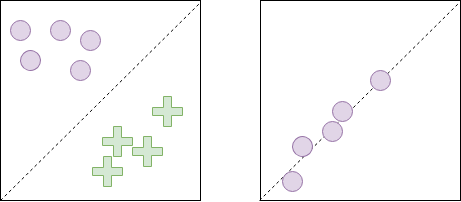
\includegraphics[scale=0.5]{figures/class_vs_reg.png}
    \caption{Left: Example of binary classification. Right: Example of regression} 
\end{figure}
  


\subsubsection{unsupervised machine learning}
\textbf{Unsupervised learning:} is the act of training without any supervision, on the sense that we do not give the algorithm the answer to the training data set. %TODO more 
Since we do not have categorised data in unsupervised learning, we often %TODO more
Types of unsupervised learning can, for instance, be clustering, the act of sorting data based on similarity.
An example of this can be if we want to sort plants based on species, or we are detecting anomalies in a dataset. Unsupervised learning can be used for PCA %TODO CITE 
or other dimensionality reduction methods.\\
A third method to used unsupervised learning is the adversarial route, where we use machine learning to make similar looking data to the original data set. 
        
\begin{figure}
    \centering
    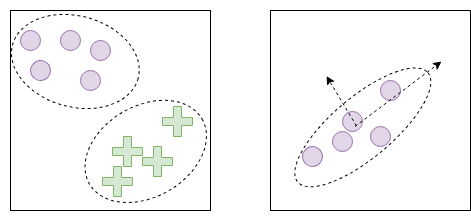
\includegraphics[scale=0.5]{figures/cluster_pca.png}
    \caption{Left: Example of binary clustering. Right: Example of principal component analysis} 
\end{figure}

In the description of supervised vs unsupervised we looked at a specific branch of machine learning: Classification. Classification is, as the name implies, the task of getting data sorted into groups of similarity. 
      
      
\begin{itemize}
    \item subsfication
    \item r to the pillcam projression 
    \item transcription/translation
    \item de-noising /finding missing inputs
    \end{itemize}
      
\subsubsection{rienforcement learning}


\subsubsection{Famous machine learning types}
Now that we have a basis on the three types of machine learning we can go into more detail on the most successful types of machine learning used both now and in the past. 
Machine learning was coined as a term as early as in the 10000 century. The first concept was of the \todo{more}


In more recent times, when the first computers came, a common type of machine learning was the K-nearest neighbour algorithm.
\todo{fast}
\todo{no training}
\todo{talk about it as a clustering method, classification}
\todo{proposed by}

\vspace{5px}

Another early adoption of machine learning was in the form of regression. Regression is the statistical concept of estimating the relationships among variables. It is in heavy use today, and one of the core concept we use machine learning for today. 
Legendre first used regression in 1805 with his method of least squares.\todo{cite} The least square methods were first done by hand, and it was at the time one best models, backed by math, to estimate the relationship between an input and a subsequent output. 
\todo{find out how much I need to write here}

Today regression analysis is widely used in statistics and informatics, and there is a significant overlap between the two research fields. While often we can make analytical models when working with a dataset with few variables, machine learning has the possibility of making much more complex models.

\vspace{5px}

A newer and applied form of supervised machine learning is the support vector machine. The original support vector machine was invented by Vladimir N. Vapnik and Alexey Ya Chervonenkis in 1963. \todo{cite} 
In 1992, Bernhard E. Boser, Isabelle M. Guyon and Vladimir N. Vapnik suggested ways to make the support vector machine work in multiclass examples by using kernels.  

A support vector machine is a form of classifier where the goal is to divide two datasets by a line that is just between the data. 


\vspace{5px} 
\todo{perhaps NN}
\todo{might be own chapter}


    
We have now discussed the general structure of the three types of machine learning. For each of the three methods we have looked at designs that utilise their form of learning, and we have shown how they can be used in the real world.
We have also looked into some successful algorithms through the ages, highlighting innovations that helped form our vast library of methods we can use to tackle problems we meet.
We will now first go more in-depth into how a general machine learning algorithm works, giving a rundown on how a simple algorithm works from start to end.
After this, we look into a more advanced example utilising a Generative adversarial network as a template.


    
\section{How machine learning works}   
\todo{tell that this is loosely based on deeplearningbook, basic machine learning}
One of the easiest to understand tasks in machine learning is the process of regression. As stated earlier, regression is a process of approximation given prior input.

We start with one of the simplest forms of approximation, namely linear approximation. In linear approximation, we are interested in finding the function that best defines our data using only a polynomial of the first degree.  First, we recall that a first-order function is always on the form
\begin{equation}
y = ax +b 
\end{equation}
Where x is input, y is output and the constants a and b  defines the function.
    
\begin{figure}
\centering
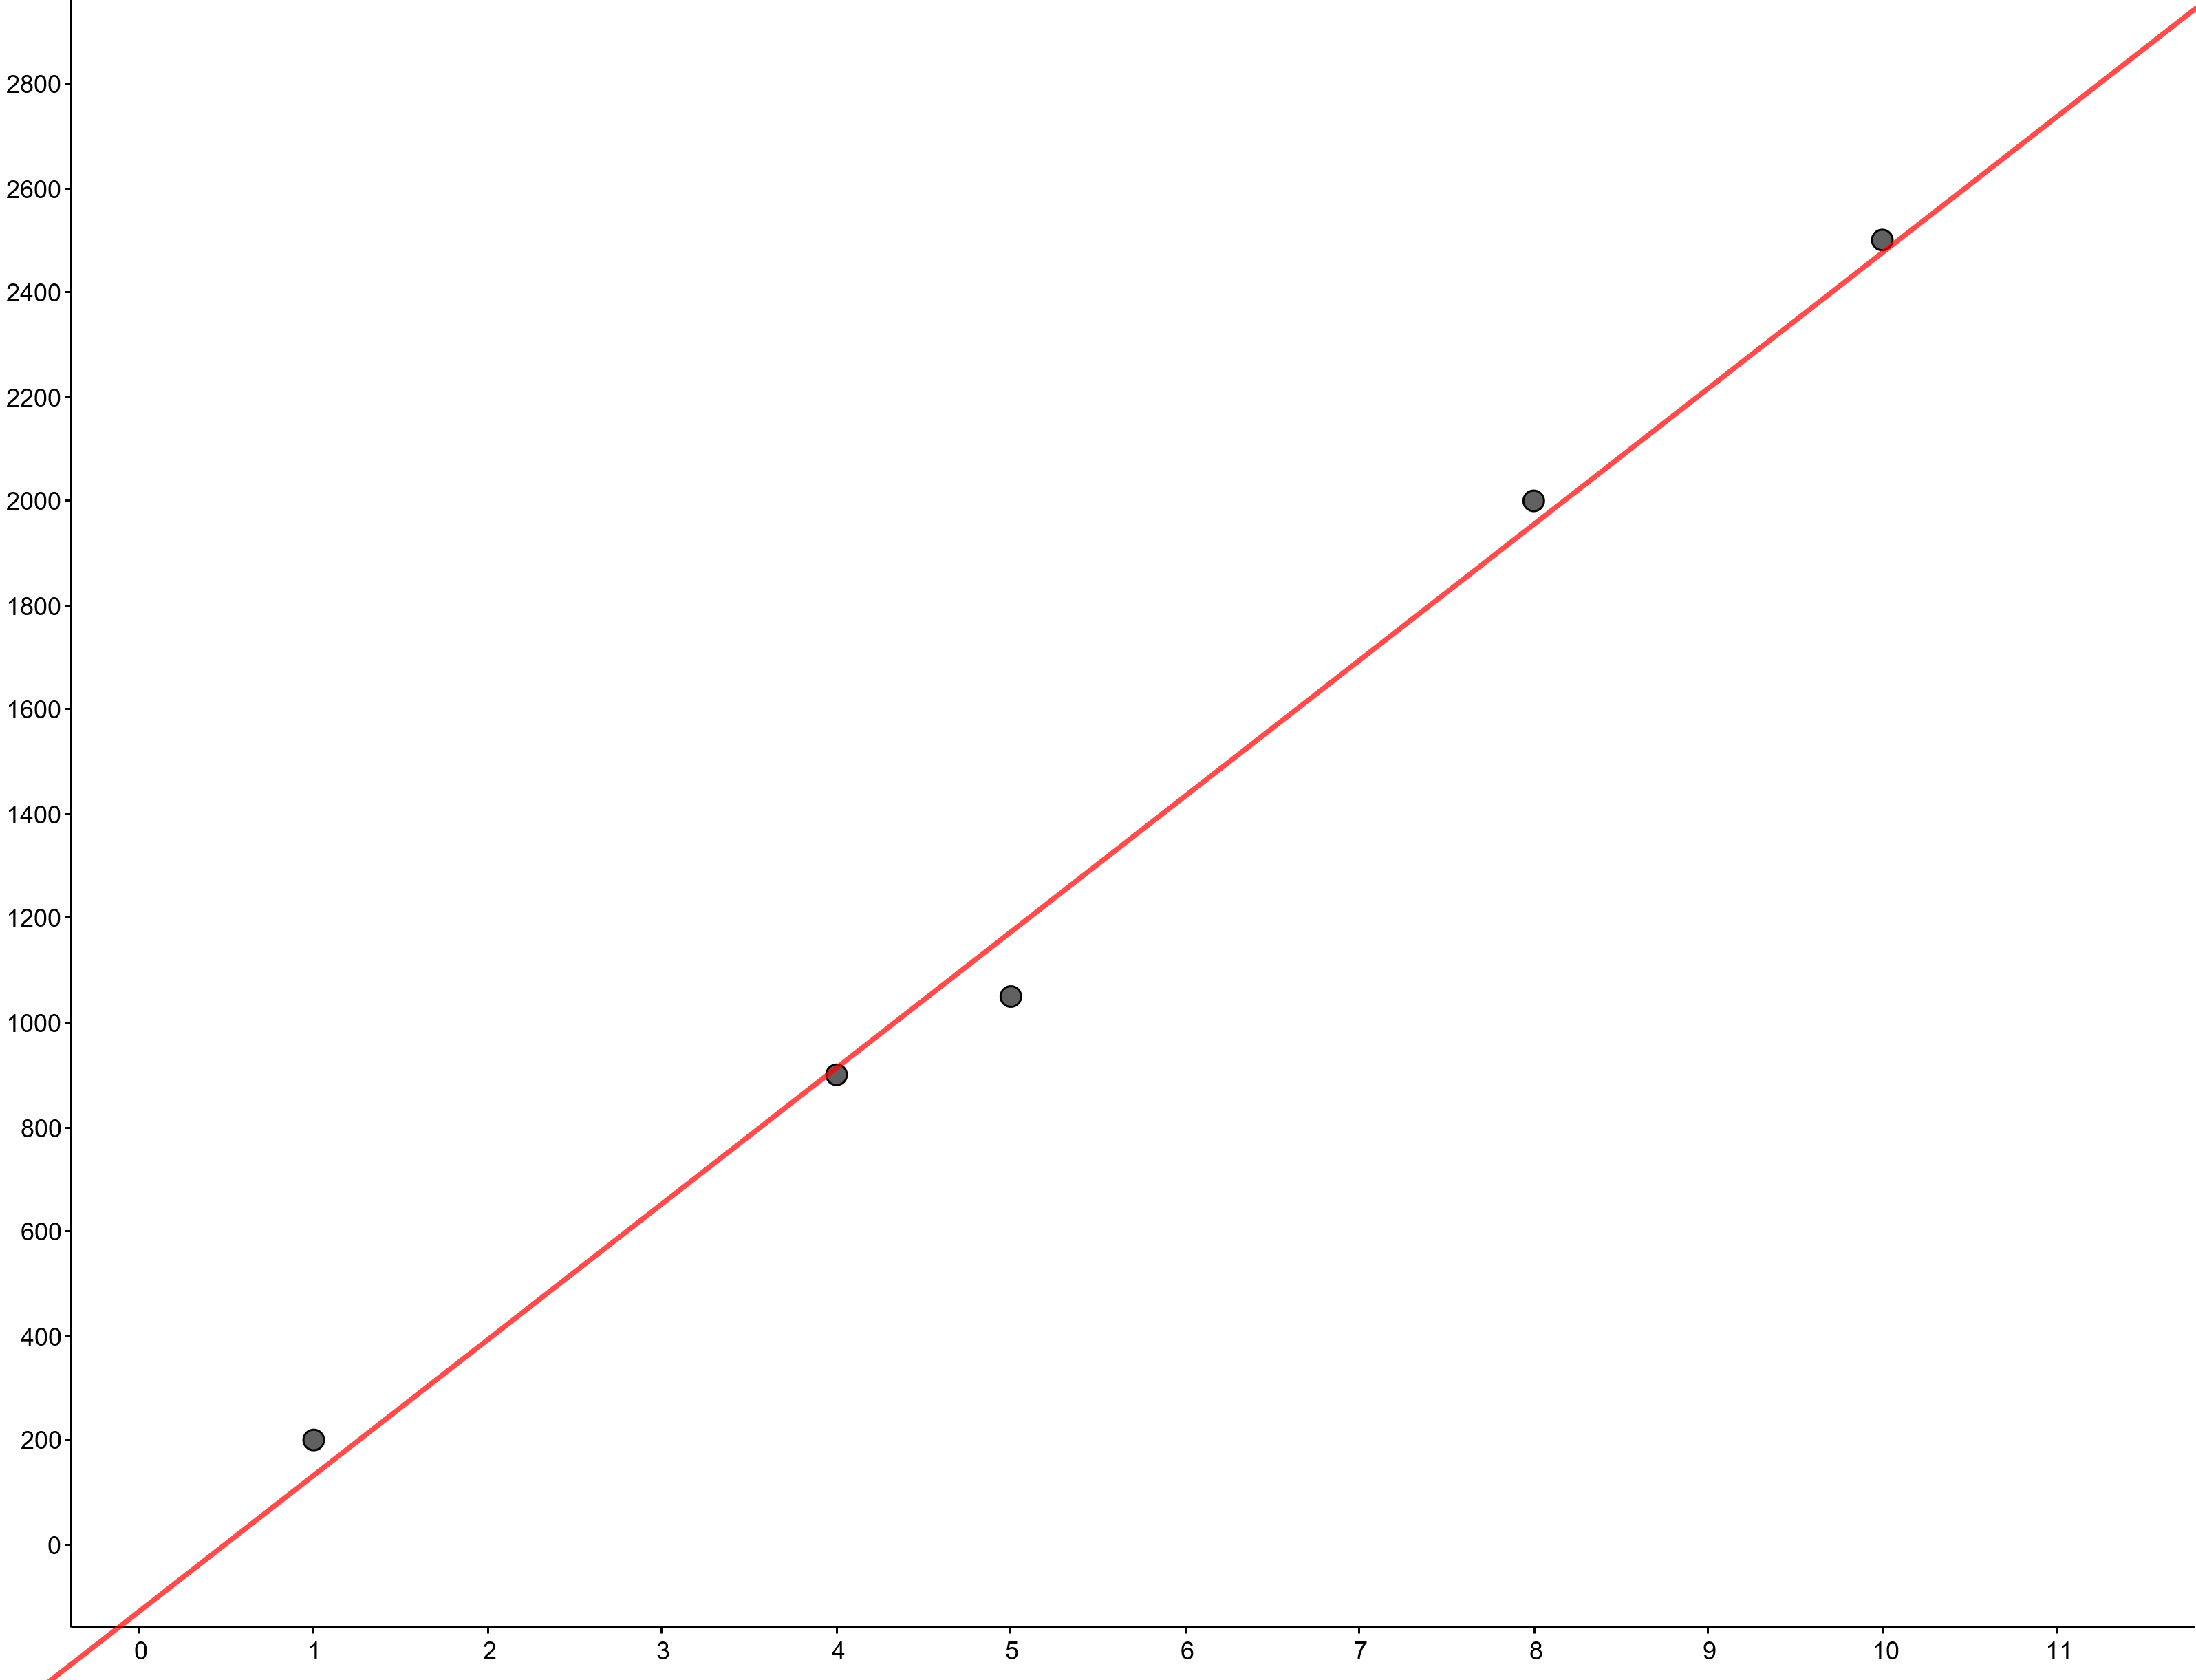
\includegraphics[scale=0.05]{background/figures/linear_regression.png}
\caption{Example of linear regression in Geogebra\todo{cite geogebra}. Here the red line is the best approxmiation of a y value, given an x value.} 
\label{fig:geogebra}
\end{figure} %credit AK for img

Figure \ref{geogebra} shows an ideal example of linear regression. Here we approximate the values of our model with the straight line defined by choosing the right slope (a) and the right constant (b).
With the knowledge of math, we look into how to do it computationally with the help of simple machine learning. 

 
We can recall from the quote by \cite{MitchellTomM1997Ml} that we gain experience E by doing a task T. In our example we choose to store our experience as its done in equation \ref{eq:ML_lin}.
    
\begin{equation}
y=W^{(1)}x+W^{(2)}\\
\label{eq:ML_lin}
\end{equation}

Here, like before, our output is y and our input is x. We have replaced a and b with new placeholders $W^{(1)}$ \& $W^{(2)}$.
Now our goal is to, given a task T, gain experience E and store it in $W^{(1)}$ and $W^{(2)}$. With our values for $W^{(1)}$ \& $W^{(2)}$ we want the best performance P.  The best performance here is defined as getting the smallest difference between the predicted output data and the actual output data. 


The most prominent way of calculating this error is to use the mean square error between the predicted and actual output of the data. 
\begin{equation}\label{MSE_form}
     MSE=\frac{1}{2m} \sum_i (\hat{y}-y)_i^2
\end{equation}
Where $m$ is the number of samples, $y$ is the real output, and $\hat{y}$ is the predicted output. The 2 in the denominator is just a constant to make the derivation of the formula easier.\\
    
From this, we can intuitively see that the error tends towards 0 when $\hat{y}$=$y$. We can also note, because of the squaring in the formula, that the error is only based on L2 distance between $\hat{y}$ and $y$.\\

Now that we have an error, we need a way to improve it \todo{more about GDEC}
At this point, we have a way to store experience E (in  $W^{(1)}$ \& $W^{(2)}$), measure performance P (in the MSE), and we have tasks T (in the form of input-output pairs).


Given an input-output pair, we will now look at how to use machine learning to better approximate the next input-output pair.

   
Lets start with: 
\begin{equation}
	x=\left[ \begin{array}{c} 1\\ 2\\ 3\\ \end{array} \right]
	y=\left[\begin{array}{c} 1.5\\2\\ 2.5\\\end{array}\right]
\end{equation}
with the weights $W^{(1)}=0$ and $W^{(2)}=0$
Using the formula \ref{eq:ML_lin} we can calculate  $\hat{y}$ to be
\begin{equation}
    \hat{y}=\left[\begin{array}{c} 0\\0\\ 0\\\end{array}\right]
\end{equation}

We can now calculate the performance by applying the mean square error function. Using \ref{MSE_form} gives us a loss of:
\begin{equation}
   \frac{1}{2*3} ({(1.5-0)}^2+{(2-0)}^2+{(2.5-0)}^2)=2.08
\end{equation}
With our new found error, we need a way to use this to update our weights $W^{(1)}$ \& $W^{(2)}$ to get a better estimate. 
    

The most common way to update our weights is to use gradient descent. 
Gradient descent is a first order iterative optimisation algorithm \todo{cite Wikipedia GD} for finding the minimum of a function. In our case, we are looking for the minimum value of the MSE function. Gradient descent is defined as (simplified for our example):
\begin{equation}
	a_{n+1}= a_{n} - \gamma \nabla F(a_{n})
\end{equation}
Where $\nabla$F() is the derivate of function in question, a is the input at step n, and $\gamma$ is a learning rate set to a small number. 

Derivating \ref{MSE_form} and using a learning rate of 1 we get the following. 
\begin{equation}
\label{MSE_deriv_w0}
     \nabla F_{W^0} = \frac{d}{d_{W^{0}} } \frac{1}{2m} \sum_i (\hat{y}-y)_i^2 \\
     \nabla F_{W^0} = \frac{1}{m} \sum_i (\hat{y}-y)_i\\
\end{equation}

\begin{equation}
     \nabla F_{W^1} = \frac{d}{d_{W^{1}} } \frac{1}{2m} \sum_i (\hat{y}-y)_i^2 \\
     \nabla F_{W^1} = \frac{1}{m} \sum_i (\hat{y}-y)_i \dot \hat{y}\\
\end{equation}

 
    
	
	
	
	\subsubsection{Feed forward}
    
	\subsubsection{Loss and gradient decent }


	

   
	  

	
\section{Neural Networks}
We have looked at different types of machine learning, and we have gone in depth into how a linear regression model works. In this chapter, we want to get further insight into how we can make more complex models, and we will look into the most popular method for machine learning, namely Neural Networks. 
After the rundown on how neural networks are built up and how they operate, we will look into convolutional neural networks. In the end, we will look at successful networks, mainly made for image classification.


\subsection{The perceptron}
To explain how a neural net operates, we first need to look at the most fundamental structure present in every type of neural network, namely the Perceptron.
The fist perceptron was introduced by \todo{who} in \todo{find when}, and it was made as an attempt to mimic the human neuron.  


\begin{figure}[h]
        \centering
        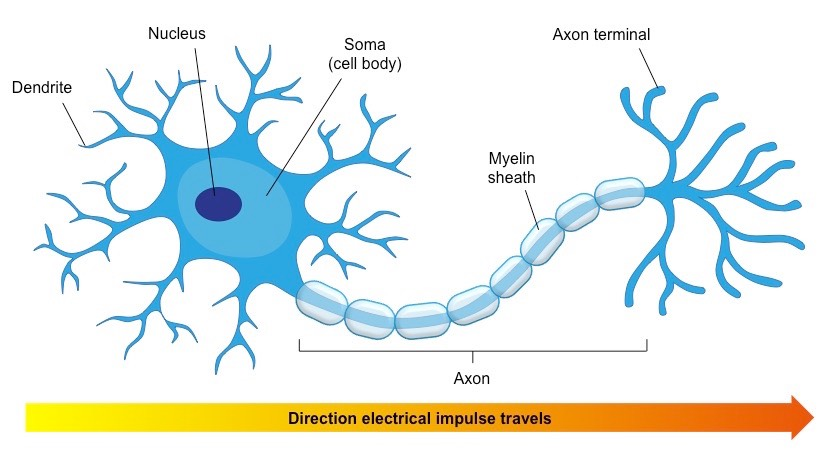
\includegraphics[scale=0.5]{background/figures/neuron.jpg}
        \caption{https://socratic.org/questions/how-is-a-neuron-adapted-to-perform-its-function}
        \label{fig:neuron}
\end{figure}



Figure \ref{fig:neuron} shows how a human neuron looks like, and in which direction the signal goes. Each neuron is connected to multiple other neurons by connecting the dendrites to other neighbouring neurons. 
When a signal is sent, the dendrites register the signal and sends it through the axon out to the axon terminal. At the axon terminal, other neurons pick up the electrical signal and pass it through their axon.
This flow of electricity is the fundamental way different part of our brain communicates, and the different pathways the signals can take represent how we learn. 

\begin{figure}[h]
        \centering
        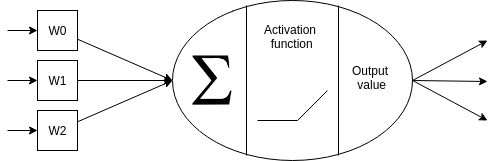
\includegraphics[scale=0.5]{background/figures/perceptron.png}
        \caption{Simple perceptron}
    \label{fig:perceptron}
\end{figure}

We can now look at the perceptron in figure \ref{fig:perceptron}, as we can discern, this mathematical model has the same structure, and we have the same flow as we would in the human brain. 
First, we get numerical data from, either other perceptrons, or from an input. We add it together and send it out on the other side. We will now look more in depth how this is done, and show how the mathematics behind it works. \\

\textbf{Step 1:} our perceptron gets signals $a_{(i,0)}-a_{(i,n)}$ where $n$ is the number of inputs to the perceptron.\\

\textbf{Step 2:} each of our signals $a_{(i,0)}-a_{(i,n)}$ is multiplied by a weight $W^{(0)}$ -  $W^{(n)}$. \\

\textbf{Step 3:} we sum every input to a scalar. \\

\textbf{Step 4:} We apply an activation function. This can be a simple sigmoid function or tanh function, but the most common is the Rectified linear unit (ReLu) \todo{cite} \\ 

\textbf{Step 5:} The output of the activation function $a_{(j,0)}-a_{(j,n)}$ is sent to the next perceptron. 

\todo{talk about why we use an activation function}



\subsection{Multilayer perceptrons}
The neural network was a proposal made by Warren McCulloch and Walter Pitts (1943) \todo{cite}  created a computational model for neural networks based on mathematics and algorithms called threshold logic. 
\todo{talk about the single neuron made by that dude}

The first multilayer network at the time used backpropagation in the same way described in \todo{find formula}.

\begin{figure}[ht!]
\centering
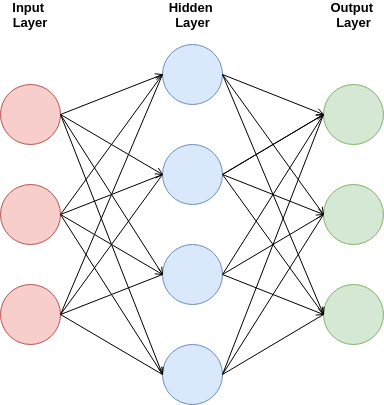
\includegraphics[scale=0.2]{background/figures/neural_network.png}
\caption{THIS IMAGE IS SHAME(LESS)LY taken from the internetz, draw own so the lawyers don't get you!}
\label{fig:mlnn}
\end{figure}

Figure \ref{fig:mlnn} shows the basic structure of a multilayer network.
In this figure, we have four things we need to look into.

\subsection{Feed forward and backpropagation through a neural network}
\todo{looked at how MLP works, let's look at back-and-forward prop}





    
\subsection{Convolutional neural networks}
The multilayer perceptron we have discussed is a strong tool that can learn a multitude of decision boundaries, and subsequently learn to classify thousands of different classes. 
As we get more data and more classes, the networks needed to solve our problem grows. We can recall from chapter \todo{ref chapter on MLP} that the number of weights between neurons is \todo{insert math}. As the number of perceptrons per layer in our neural networks increases, the total amount of storage space increases by a factor of 4 \todo{fix this}

Another problem with the standard MLP is the fact that it is spatially dependent. Given an input $x$, the output, $y$, of the MLP will vary a lot if we shift the input data by one place, or if we flip the data. In some cases, this is something we want in our machine learning algorithms, but more often than not, this behaviour is not a desirable outcome.

Given the downsides we have with regards to memory usage and non-spatiality in our multilayer perceptrons, we present Kunihiko Fukushima \todo{cite} solution to solve both complications.

Convolutional neural networks are the most popular form for image recognition, segmentation, and classification \todo{cite, IEEE paper got cites}

\todo{transition}

Convolutional networks work with filters and assign a weight to each pixel in the filters used. This use of filters significantly reduces the number of weights between layers, since we now have weights that are not dependent on the input size, and only dependent on the size and number of filters.

\todo{sliding window}

Given a $5x5$ filter 

\begin{figure}[ht!]
        \centering
        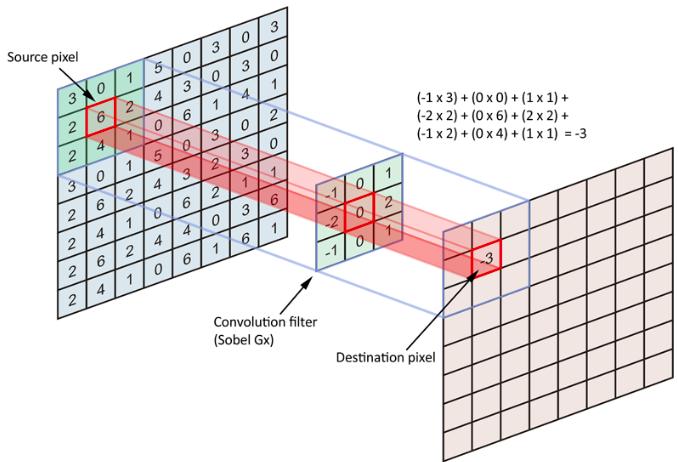
\includegraphics[scale=0.2]{background/figures/conv_neural_network.png}
        \caption{THIS IMAGE IS SHAME(LESS)LY taken from the internetz, draw own so the lawyers don't get you!}
    \end{figure}
 
\todo{the layer structure}

\subsection{Additional layers}
\subsubsection{Activation layers}
\subsubsection{Pooling}
\subsubsection{Normalisation}
\subsubsection{Dropout}


\section{Neural Network models}

    \subsection{Autoencoders}\label{Explaining_autoencoders}
	  %%TODO CITE: http://www.deeplearningbook.org/contents/autoencoders.html
As we recall from earlier, an autoencoder is a type of neural network that tries to output a recreation of the output.\todo{we are not recalling} \\ 

We can do this by having an encoder, $h=f(x)$, connected to a decoder, $r=g(h)$. 
An autoencoder has the job to set $g(f(x))=x$ over the whole input, but in most cases this is not a practical program. We often gives the autoencoder the restriction
that it has to map the input through a latent space that has a smaller dimension than the input dataset.\\
This is called an undercomplete autoencoder.\\
\vspace{10px}
\begin{figure}[ht!]
	\centering
	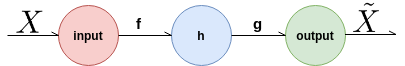
\includegraphics[scale=0.5]{background/figures/SimpleAE.png}
	\caption{The general structure of an autoencoder, mapping $\textbf{x}$ through $\textbf{h}$ to an output $\textbf{r}$.}
\end{figure}

As with supervised classifiers we can use gradient decent to optimize the model. This is because we are trying to recreate the input $\textbf{x}$ from out output $\widetilde{\textbf{x}}$\\
	  
This can simply be done by minimizeing the loss function\\
\begin{equation}
	L(\textbf{x},g(f(\textbf{x})))
\end{equation}

with for instance MSE with gradient decent. \todo{explain MSE, and general loss on an ealier time}\\
Now we can transfer this to a more relevant example by making an image as input and use convolutions to reduce the dimensionality in the encoder and increase the dimentionality in the encoder.
\begin{figure}[t]
	\centering
	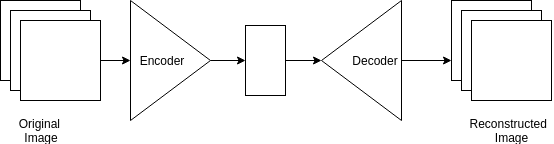
\includegraphics[scale=0.5]{background/figures/CAE.png}
	\caption{Convolutional autoencoder with an RGB image as input, and the reconstructed image as output.}
\end{figure}
	
    \subsection{Advaserial neural networks}
\paragraph{This is explaining GANS, put me in the right place} %%TODO CITE: http://www.deeplearningbook.org/contents/generative_models.html and Goodfellow at al. 2014
Now that we have looked at autoencoders we can take it a step further. 
generative advaserial models can be used as a generator of new data, and can have som reseblance to autoencoders \ref{Explaining_autoencoders}, especially variational autoencoders %TODO cite VAE, ref VAE

The difference lies in that advaserial networks is based on game theoretic scenarios in which a generator network is compeating agenst an advasery. 
The generator produces samples $x=g(z;\theta^{(g)})$, where $g$ is the network given the weights $\theta$. Then the discriminator network predicts if a sample is drawn from the dataset or from the generator.
More spessific, it gives a probably given by $d(x;\theta^{(d)})$ , and determins if $x$ is from the generator or the data-set. 
Since we have two networks compeating agenst each other we can look at this as a Zero-sum game with the generators payoff is determined by $v(\theta^{(g)},\theta^{(d)})$, and the discriminators payoff is determined by $-v(\theta^{(g)},\theta^{(d)})$.
\textit{$v$ is here a function that is determined by both the sucsess rate of the discriminator and the generator, the most common used is}
\begin{equation} %TODO: CITE First gan paper on formula
	v(\theta^{(g)},\theta^{(d)}) \; = \; \mathds{E}_{x\sim p_{data}}\log{d(x)} + \mathds{E}_{x\sim p_{model}}\log{(1 - d(x))} 
\end{equation}
as derived from Goodfellow et al. %TODO cite 
	  
Lets look at a gan in detail. \\
\begin{figure}[ht!]
	\centering
	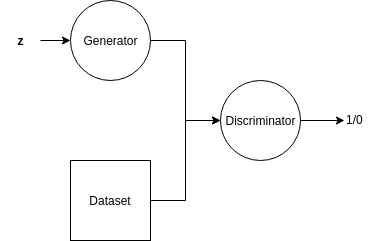
\includegraphics[scale=0.5]{background/figures/simpleGAN.png}
	\caption{The idea behind a GAN. Here the generator saples from a random (Gaussian) distribution and generates samples that the discriminator classifies as real or fake}
\end{figure}
	
\subsubsection{UCNN?}	
\subsection{Recurrent neural networks}
\subsubsection{LSTM}

\subsection{Contextencoders}
Inpainting can also be done with advaserial models, and using a network trained to do the task of inpainting can be a lot more powerful than using just an autoencoder\todo{ref} or the naive methods\todo{ref}.
A contextencoder is building on the advaserial principle by using a generator/discriminator pair to fill in masked areas in an image. 
	
The concept behind a Contextencoder is to take the whole image as input to an encoder/decoder pair and \todo{finish}
     
\subsection{CC-GANS}  
\subsection{Pixel CNN}
      
    



	    
	  
\section{Explain how the ML-methods can be used with the polyps}
	When you work with machine learning a lot of the job is to make the data as clear as possible. \\
	Imagine that you want to do something simple as reading an analogue clock. The \"straight forward\" way to do it is to  
	make a convolutional neural network to look at the dials. This will require a much more complex network compared to if you could convert the angle of the dials
	to degrees and have that as an input to your model.

	\begin{figure}[ht]
	  \centering
	  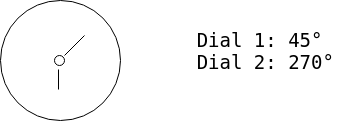
\includegraphics[scale=0.5]{methods/figures/Clock.png}
	  \caption{A clock needs a more complex network compared to just the degrees}
	\end{figure}
	%TODO FIND ORIGinal source
	The trick is often to make the data as refined as possible. 
	Further some of the techniques used is described.
	
	\todo{Here i need to talk about how preproccesing might help the problem, and make this a springboad in to the next section: the problem at hand}
	
	
	\todo{adress the problem with lack of data, and talk about how machine learning can help, machine learning.}
	  
	  
\section{The problem at hand}
	  Now that we have the definition of machine learning and the current task, we can focus on the task at hand; finding polyps. In an ideal world\footnote{Ideal as in the only disease we could get in  the GI tract was cancer originating
	  from polyps which looked exactly the same} we have a
	  Classification problem with only two classes: Non-polyp and polyp. 
	  
	  \begin{itemize}
	    \item SVM 
	    \item CNN 
	    \item random forests
	    \item knn
	  \end{itemize}

\iffalse
\section{In painting}
  We have discussed the importance of good input data, and the potential benefits to resource usage and ease of making a good model.
  So a priority when it comes to image classification is to have data without anomalies and other areas that can be interpreted as a feature for the classifier. 
  In a machine learning perspective, the data is best if it has the same structure, and is %TODO similar enough.
  In painting is the process of reconstructing lost or deteriorated parts of images and videos. %TODO CITE https://en.wikipedia.org/wiki/Inpainting
  

  From prior papers on polyp detection in the GI tract %TODO CITE!!!
  we have clear results that the black corners, and the green squares trigger a big activation %TODO WRITE BETTER
  when it comes to classifying images. 
  From %TODO CITE, find out who
  's paper, we can see that the activation map on a regular image gives very high result on, in addition to the polyp, the corners and the green sqare. 
  \begin{figure}[ht]
    \centering
    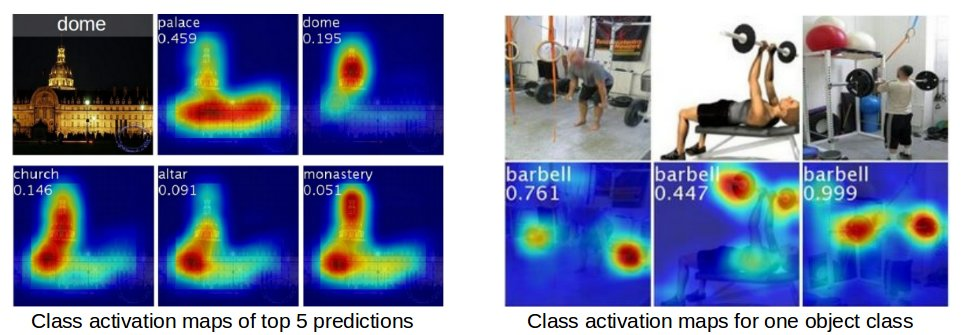
\includegraphics[scale=0.5]{background/figures/placeholder.jpeg}
    \caption{Using X's activation map we can see that the edges triggers unwanted activations}
  \end{figure}
  
  In addition to sqares and edges, we also have the problem that parts of the image is over saturated at points where the light from the led is reflected directly back to the camera.
  Another problem is when the camera captures images that are too close to the wall. Both of these scenarios creates patches where the saturation is maximum. 
   \begin{figure}[ht]
    \centering
    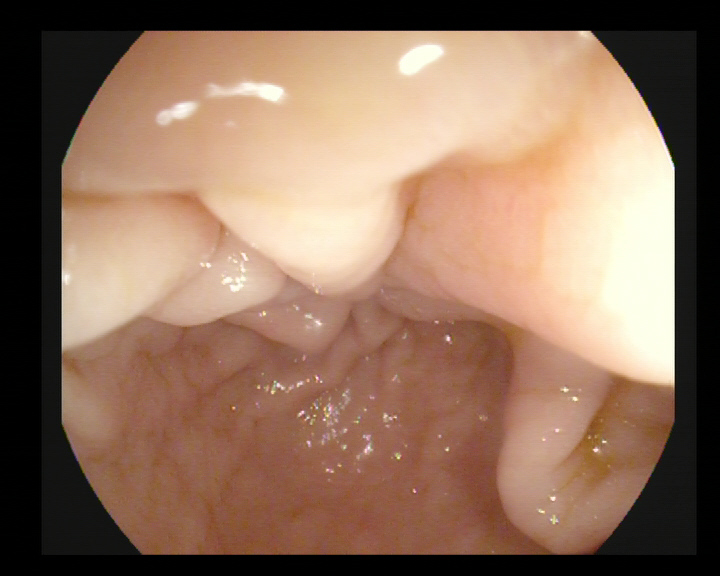
\includegraphics[scale=0.5]{background/figures/reflection.jpg}
    \caption{we have two different types of saturation: the reflected area in the top part of the image, and the right side of the image.}
  \end{figure}
  in an ideal scenario the image would have no pixel values at max, and as little frame as possible. 
  We therefor want to make a tool that can help us with this.
  \subsection{Naive methods for In painting}
    Inpainting is not a new area of research, as it has been around since %TODO CITE
    Because of this there are many naive methods that gives good inpaintings. 
	
    \subsubsection{Textured syntesys based on image inpainting}
    \subsubsection{MOARE}
    \subsubsection{MOARE}
   \subsection{Naive methods for borderfinding}

%
% THIS SECTION MUST BE MOVED/FIXED
%
\section{Naive Methods REM}
	  Now that we have an idea of what we are looking for we can first turn to some more naive methods for detecting anomalies, and for enhancing the images.\\
	  The field of image processing has been researched since\\ %TODO WHEN
	  
	  Using some of the classic methods in image processing we can see if\\ %TODO
	  
	  We often describe the method in to two groups of information: First and Second order statistics.\\
	  \textbf{First order:} First order statistics does not take in to account the relative positioning of the pixels in the image, and because of this, gives much less
	  information than the second order statistics.\\
	  Example of First order statistics is often what information we can get out of a histogram. This can be scewness, variance, and mean value.\\
	  
	  \vspace{10px}
	  
	  \textbf{Second order:} Second order statistics takes in to account the relative positioning of the pixels in the image. We can calculate the GLCM matrix and get a much more detailed 
	  view of the image. \\
	  
	  
	  
	  \subsection{GLCM}
	    A GLCM (Grey-level co-occurrence matrix) is a matrix that is used when examining the spatial relationship of pixels in a texture. 
	    The calculation of a GLCM gives us how often pairs of pixels with spesific values and a specified spatial relationship occur at a given place in an image. %TODO CITE
	  
	    \subsubsection{Algorithm}
	      For simplicity we use only greyscale in this example:
	      \begin{figure}[ht]
		\centering
		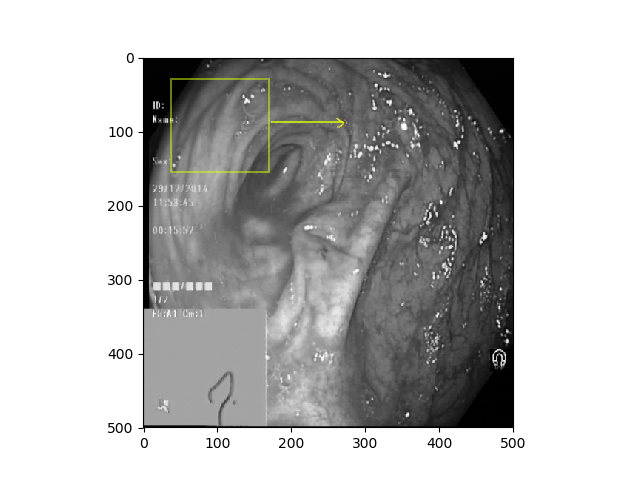
\includegraphics[scale=0.5]{figures/sliding_window_box.png}
		\caption{GLCM capturing features}
	      \end{figure}
	      The algorithm starts by running a sliding window over the image, often with a stride, and for each stops calculates the spatial relationship between each pixel specified.
	      The result can be something like this figure %TODO link to figure
	      where we can read out the most likely neighbouring pixel.
	       \begin{figure}[ht]
		\centering
		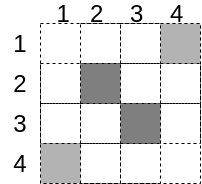
\includegraphics[scale=0.5]{figures/Simple_GLCM.png}
		\caption{GLCM Matrix}
	      \end{figure}
	      The darker colours on in the matrix is indicating that we often have a jump between, for instance pixel-value of 1 and a pixel-value of 4, but no from 1 to 1.\\
	      With this information we can get a naive pattern-recogniser. 
	    \subsubsection{Other uses}
	      Besides for the pattern recognition we can use the GLCM to get the information on:
	      \begin{itemize}
	       \item \textbf{Contrast} is the difference in luminance or colour in the picture. We would expect low contrast in the “background” and higher contrast around edges and irregular objects.
	       \item \textbf{Homogeneity} is how similar a local area is to itself
	       \item \textbf{Variance} $\sigma^2$ , is directly a measure of ”roughness”
	       \item \textbf{Mean} value of a GLCM can give us areas with higer or lower pixel values. Good way to find polyps if they are lighter than the tissue around.
	       \item \textbf{Entropy}
	       \item \textbf{Energy}
	      \end{itemize}


	  
	  \subsection{Edge detection}
	    Using Edge detection in is another viable way to look for polyps. 
	    \begin{figure}[ht]
	      \centering
	      \begin{minipage}[b]{0.45\textwidth}
		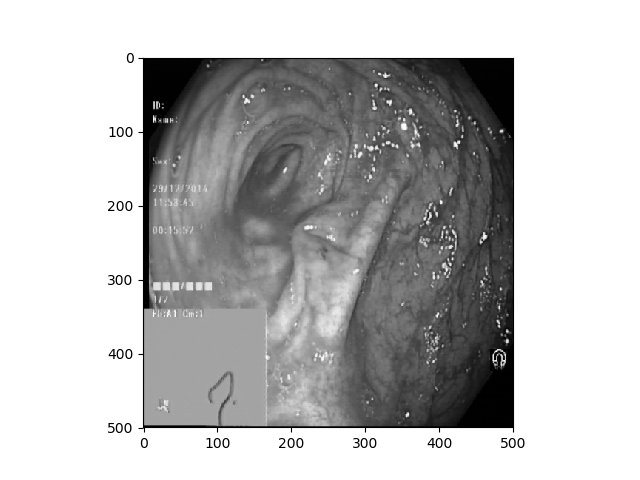
\includegraphics[width=\textwidth]{figures/sliding_window.png}
		\caption{Original image}
	      \end{minipage}
	      \hfill
	      \begin{minipage}[b]{0.45\textwidth}
		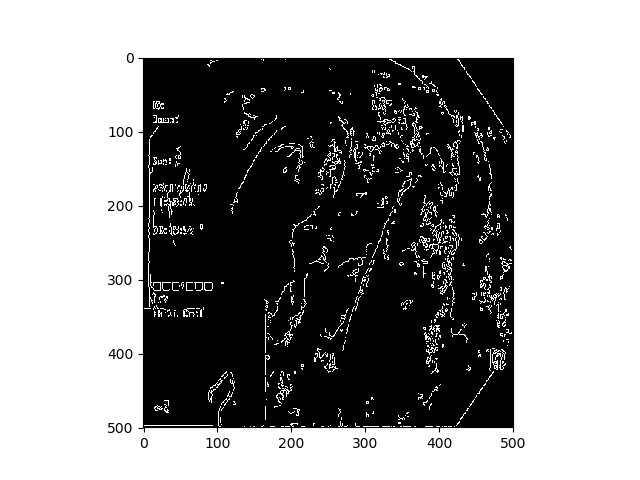
\includegraphics[width=\textwidth]{figures/Canny.png}
		\caption{Edges of the picture}
	      \end{minipage}
	    \end{figure}
	    \subsubsection{Algorithm}
	      For each pixel look at the neighbouring pixel, if \\
	      
	      \begin{centering} 
		$ abs(p_a - p_b)>tresh $\\ 
	      \end{centering}
	      
	      then mark pixel as an edge pixel. \\
	      
	  \subsection{Hough Transforms}
	    Using for instance Canny edge detection %TODO CITE
	    we can get a better view of where the potential border of the polyp/anomaly is. (As shown in %TODO FIG CITE)
	    
	    A hough transform can i theory have many/any shape(s), and together with edge detection, we might find some of the polyps this way.
	    
    
    
    
    
    
	
    As we can see from this, there are a lot of old methods that can give approximations. We can also conclude that none of these methods are perfect.
    We will therefore look at methods that takes learning in to use.
\section{Using machine learning for inpainting}
    \subsection{AE}
    \subsection{CE}
    \subsection{CCGAN}
    \subsection{PCNN}
    As discussed earlier, machine learning is using prior experiences to make decisions given the problem at hand. 
    It is also worth mentioning that we do not need labeled data, since we are in a way looking at a global average of every image both with, and without polyps. We are therefor incentiviced to use an 
    Unsupervised approach.
    Since machine learning is learning from a training set, it is important that the training set contains as little as possible of the features we want to remove. \\
    
    Because of this the first thing we need to do if we are going to mask out corners and sqares, is to limit the training set to only contain cropped, non-sqare images. 
 
    \begin{figure}[ht]
      \centering
      \begin{minipage}[b]{0.45\textwidth}
	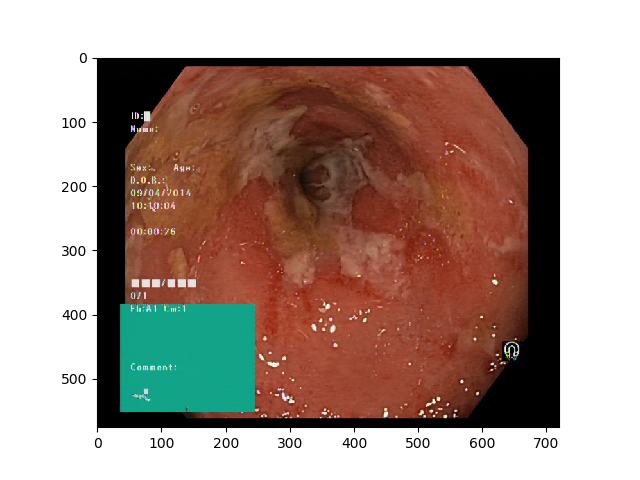
\includegraphics[width=\textwidth]{background/figures/uncropped_img.png}
	\caption{Original image with black padding}
      \end{minipage}
      \hfill
      \begin{minipage}[b]{0.45\textwidth}
	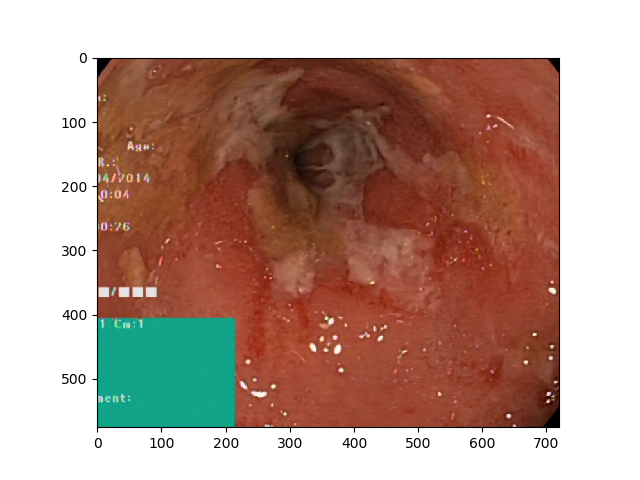
\includegraphics[width=\textwidth]{background/figures/cropped_8percent_img.png}
	\caption{Black edges cropped away + 8\% zoom}
      \end{minipage}
      \caption{Here we have an example on how we would make an image better to train on. This is not representative of the training, since we only use images without the green square under training}
    \end{figure}
    
    Now that we have better images to train our data with, we need the correct algorithm.
    We have already seen unsupervised learning aproaches in chapter %TODO ref 
    \newpage
    \subsubsection{Algorithm}
      \todo{Hvordan skal jeg gaa frem nar det kommer til aa presantere disse? skal jeg bare si hvilke metoder jeg har testet?}
      Text about presenting UML, and stuff.
  
	\newpage
	As we recall from earlier, an autoencoder is a type of neural network that tries to output a recreation of the output.\\%TODO: REF the part about autoencoders 
	We can use this for inpainting by setting the algorithm to train on images with areas cropped away.
	There are a couple of different way we can train an autoencoder to do this.\\
	
	%\todo{should i talk about the different ways or present the best?}
	
	
	\vspace{10px}
	\textbf{Denoising Autoencoder with MSE loss:}\label{par:Denoising_Autoencoder_with_MSE_loss}\\
	The simplest way to train the autoencoder is to first take the trainingset $\mathds{X}$ and make an augmented copy $\widetilde{\textbf{x}}^{(i)}$ for 
	every data point in $\textbf{x}_{\sim \mathds{X}}^{(i)}$. \\
	\textit{Here $\widetilde{\textbf{x}}$ is a copy of x with random areas masked.}\\
	
	Now we minimize the loss function\\	
	  \begin{equation}
	    L(\textbf{x},g(f(\widetilde{\textbf{x}})))
	  \end{equation}
	over the whole image.\\
	\vspace{20px}
	
	With this approach the autoencoder learns to fill in the blank spots with plausible data, without changing the rest of the image. 
	\todo{this will probably work best if the autoencoder is not undercomplete, perhaps talk about this}
	One problem by this approach is that we do not want the rest of the image to change for obvious reasons, and the alogrithm as it is here has the flaw that it will change all the pixels in the image, at 
	least to a minor degree. \\
	
	This can be somewhat fixed by only taking the augmented parts, and pasting the directly in to the image. This will leave most of the original image, except for the parts that was cropped randomly.\\
	
	\vspace{10px}
	\textbf{Denoising Autoencoder with \todo{clever tittle}:}\\
	If we take what we learned from \ref{par:Denoising_Autoencoder_with_MSE_loss}, we can make a more optimal autoencoder:
	Rather than taking a loss like 	
	\begin{equation}
	  L(\textbf{x},g(f(\widetilde{\textbf{x}})))
	\end{equation}
	over the whole image, we can rather just focus on the parts that matters, namely the cropped areas.\\
	
	If we add the cropped image to the output from the autoencoder to make an image image, we can use this new image to train out loss.
	For most of the image, the loss will be zero, since the only part that is changed is the cropped area. 
	We can also make a new loss that is more optimal for the task at hand. 
	\begin{equation}
	  MSE_{crop}\:=\: \frac{1}{n}
	  \begin{cases}
	      \begin{array}{lcl}
	      (\widetilde{\textbf{x}}-\textbf{x}) \; if \; \widetilde{\textbf{x}} \: \in \: \textbf{x}_{crop} \\
	      0 \; else
	      \end{array}
	  \end{cases}
	\end{equation}
	Where $\textbf{x}_{crop}$ is the area that was cropped away from the original image and $n$ is the number of pixels in that area.\\
	With this modified MSE we are assured that only the pixels in the cropped area is changed with gradient decent, and we save a lot of computation as an added bonus.
	
	
	\todo{token to not train}
	\begin{figure}[ht!]
	    \centering
	    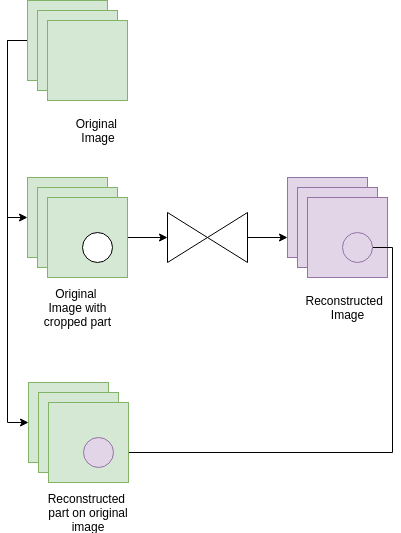
\includegraphics[scale=0.5]{background/figures/AE_for_inpainting.png}
	    \caption{Final result of the autoencoder used in the testing}
	\end{figure}
	
	
	
	
	
      \subsubsection{Explaining GANs, this will be moved}
      
	
      \subsubsection{Contextencoder}
	Inpainting can also be done with advaserial models, and using a network trained to do the task of inpainting can be a lot more powerful than using just an autoencoder\todo{ref} or the naive methods\todo{ref}.
	A contextencoder is building on the advaserial principle by using a generator/discriminator pair to fill in masked areas in an image. 
	
	The concept behind a Contextencoder is to take the whole image as input to an encoder/decoder pair and \todo{finish}
	
	
	
      \subsubsection{CCgan}
      \subsubsection{PixelCNN}
      
\fi

  
 
